\subsubsection{Benefit of GHCP vs HCP.}
Here, we compare two procedures and conduct the following experiments:

\begin{enumerate}[label=(\roman*)]
    \item Restricted GHCP from Algorithm \ref{alg:dhcp} with $\eta=0.5$.
    \item Baseline HCP, which ignores the observed test-group samples.
    
\end{enumerate} 

\paragraph{Non-triviality when baseline intervals are infinite.}
We first consider equal reference-group sizes $N_j\equiv 21$, $j\in[K]$, at test level $\alpha=0.05$. The results are shown in Table~\ref{tab:dhcp-hcp-alpha005}. In this setting, baseline HCP returns trivial (infinite) prediction sets, because the weight $1/(K_1+1)=1/11$ that \eqref{eq:hcp-measure-main} places at $+\infty$ exceeds $\alpha=0.05$. Even standard split conformal prediction applied within the test group leads to trivial prediction sets for $o\le 20$, once half of the initial sample is reserved for training.

By contrast, GHCP can return non-trivial prediction sets once the initial test-group sample is large enough. Indeed, the weight at $+\infty$ in \eqref{eq:donor-measure} is $(N_{J_0}-o)/(|S_\eta|L_{K+1})$, so the GHCP set is finite whenever $(N_{J_0}-o)/(|S_\eta|L_{K+1})\le\alpha$. In the fixed-size experiment, $N_{J_0}=21$, $|S_\eta|=10$, so the condition becomes $(21-o)/\{10(21-\lfloor o/2\rfloor)\}\le 0.05$, which holds for $o\ge 14$. Since most competing procedures produce infinite intervals in this regime, we report the numerical summary in Table~\ref{tab:dhcp-hcp-alpha005} and omit coverage and width boxplots.

\begin{table}[h]
\centering
\caption{Empirical coverage and mean interval width for GHCP across test-group size $o$, together with HCP, for fixed $N_j=21$, $\gamma=5$, and $\alpha=0.05$, using a random forest global predictor. Entries are means across $1000$ simulation repetitions, with standard errors in parentheses. Width entries equal to $+\infty$ indicate that all reported intervals were trivial.}
\label{tab:dhcp-hcp-alpha005}
\small
\setlength{\tabcolsep}{6pt}
\begin{tabular}{lcccccc}
\toprule
& \multicolumn{5}{c}{GHCP} & HCP \\
\cmidrule(lr){2-6}
Value of $o$ & 0 & 5 & 10 & 15 & 20 & -- \\
\midrule
Coverage ($1-\alpha=0.95$)
& 1.000 (0.0)
& 1.000 (0.0)
& 1.000 (0.0)
& 0.983 (0.004)
& 0.955 (0.007)
& 1.000 (0.0) \\
Mean Width
& $+\infty$
& $+\infty$
& $+\infty$
& 13.633 (0.081)
& 9.418 (0.054)
& $+\infty$ \\
\bottomrule
\end{tabular}
\end{table}

\paragraph{Width gains when all intervals are finite.}
Next, we keep the same fixed reference-group sizes $N_j\equiv 21$ and latent intercept $\gamma=5$, but increase the test level to $\alpha=0.1$. In this regime, baseline HCP has finite intervals, so the comparison is primarily about efficiency. Figure~\ref{fig:N21-cov-width-20} shows the coverage and width boxplots for GHCP across different values of $o$, and Table~\ref{tab:dhcp-hcp-alpha01} gives the corresponding summary. 

\begin{figure}[h]
    \centering
    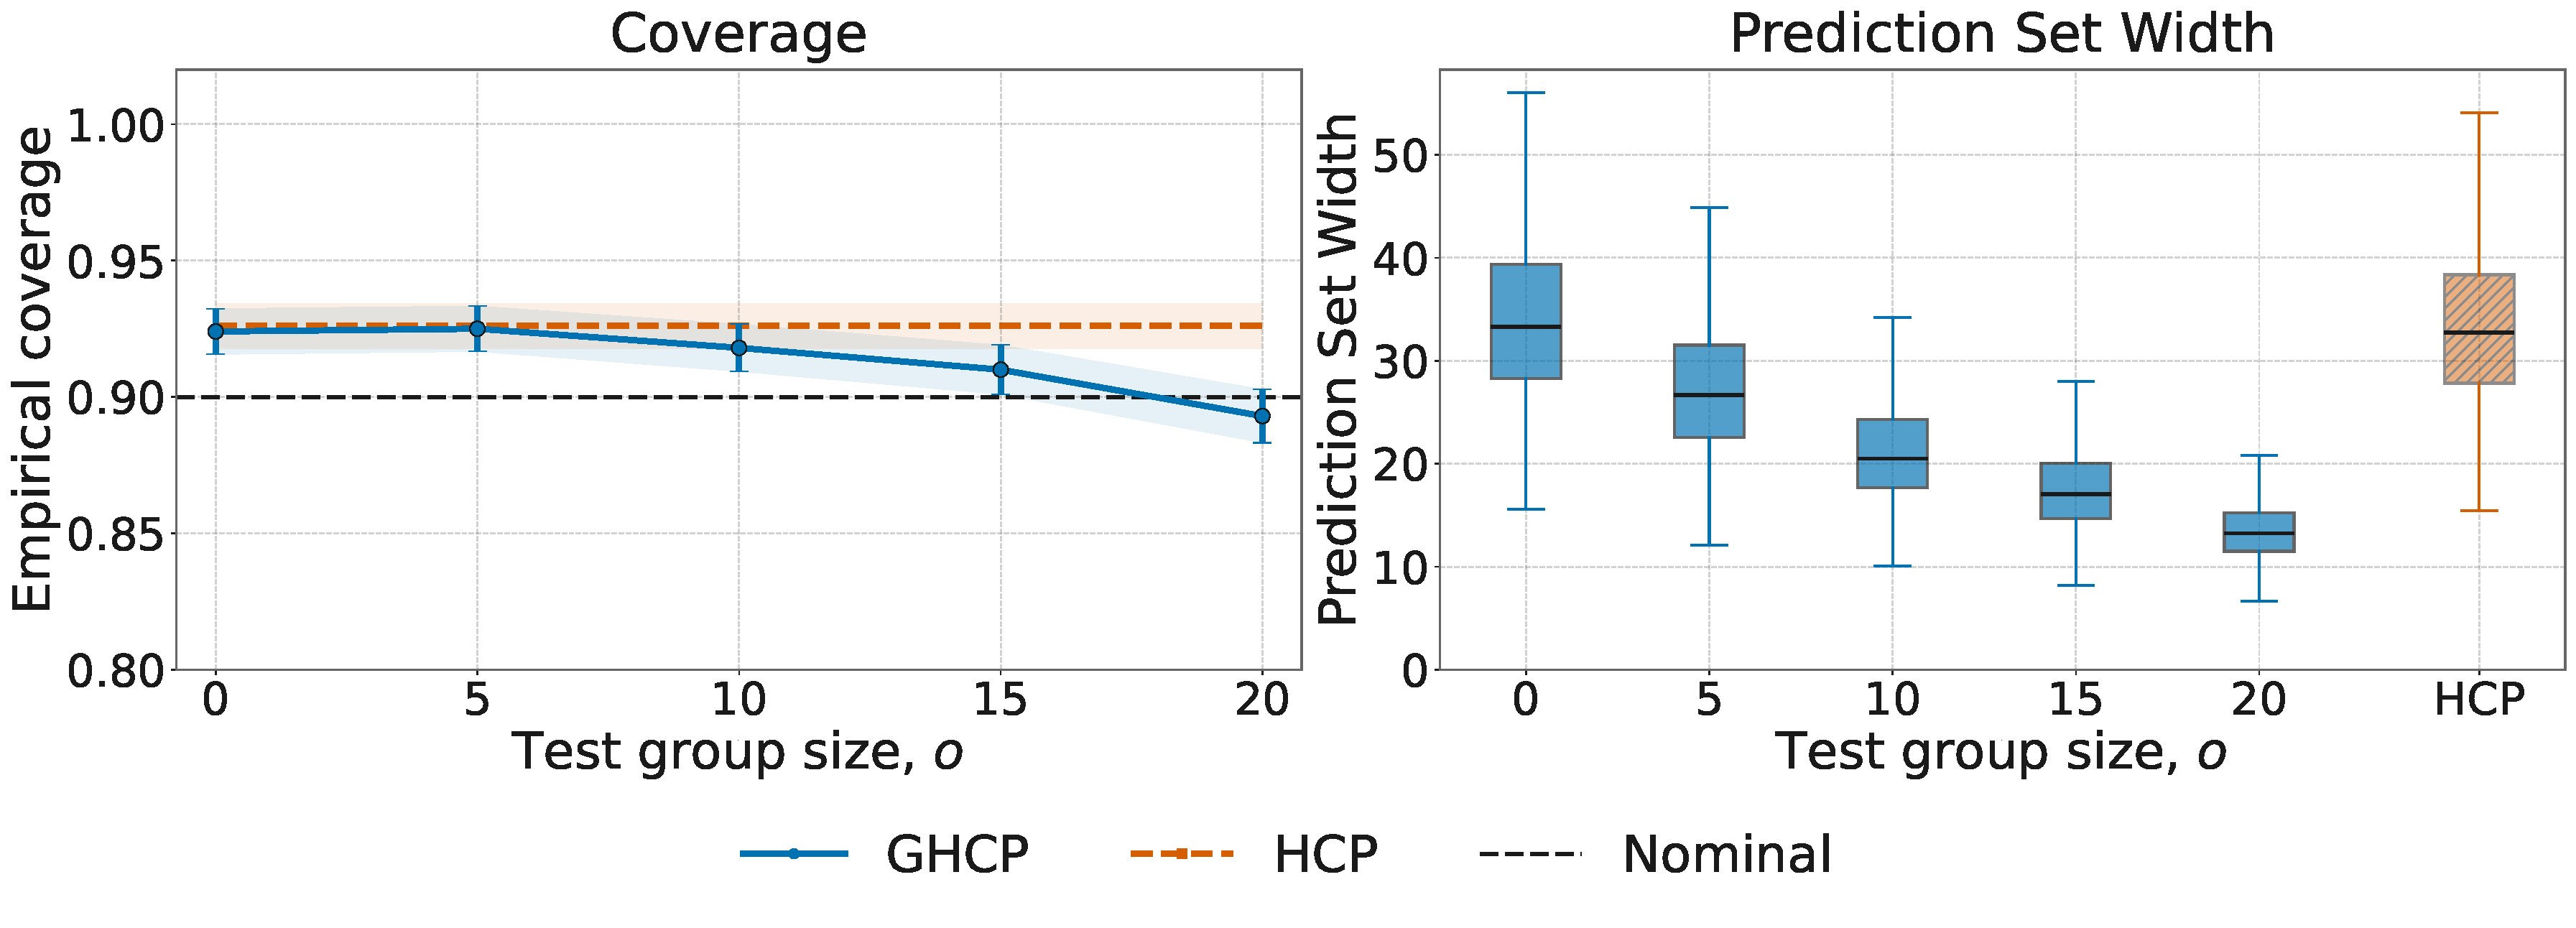
\includegraphics[width=1\linewidth]{paper-results/dgp_true_marginal_rf/figures/fixedN21_alpha0p1_coverage_width_by_o.pdf}
    \caption{Empirical coverage and width for HCP and GHCP with $o\in\{0,5,10,15,20\}$, using a random forest global predictor. Here $K=20$, $N_j\equiv 21$, and $\alpha=0.1$.}
    \label{fig:N21-cov-width-20}
\end{figure}

\begin{table}[t]
\centering
\caption{Empirical coverage and mean interval width for GHCP across test-group size $o$, together with HCP, for fixed $N_j=21$, $\gamma=5$, and $\alpha=0.1$, using a random forest global predictor. Entries are means across $1000$ simulation repetitions, with standard errors in parentheses.}
\label{tab:dhcp-hcp-alpha01}
\small
\setlength{\tabcolsep}{6pt}
\begin{tabular}{lcccccc}
\toprule
& \multicolumn{5}{c}{GHCP} & HCP \\
\cmidrule(lr){2-6}
Value of $o$ & 0 & 5 & 10 & 15 & 20 & -- \\
\midrule
Coverage ($1-\alpha=0.90$)
& 0.943 (0.007)
& 0.946 (0.007)
& 0.942 (0.007)
& 0.929 (0.008)
& 0.904 (0.009)
& 0.935 (0.008) \\
Mean Width
& 33.446 (0.256)
& 20.874 (0.151)
& 13.474 (0.089)
& 10.434 (0.064)
& 7.925 (0.042)
& 33.452 (0.260) \\
\bottomrule
\end{tabular}
\end{table}




When $o=0$, GHCP nearly coincides with HCP, as there are essentially no test-group samples to exploit. The conservativeness of HCP as observed in Fig. \ref{fig:N21-cov-width-20} can be traced to the calibration threshold. The finite calibration scores in \eqref{eq:hcp-measure-main} receive weight $1/\{(K_1+1)N\}$ each. With $K_1=10$ calibration groups of common size $N=21$ and $\alpha=0.1$, the HCP threshold is the order statistic of rank $r_{\mathrm{HCP}}=\left\lceil 0.9\,(K_1+1)N\right\rceil=208$ among the $K_1N=210$ finite calibration scores, roughly their $99\%$ percentile.

For restricted GHCP with $\eta=0.5$, the donor pool contains $10$
reference groups. After donation, nine reference groups remain for
calibration together with the partially observed test group. The GHCP
threshold is the order statistic of rank $r_{\mathrm{GHCP}}(o)=\left\lceil
0.9\cdot 10(21-\lfloor o/2\rfloor)\right\rceil$ among $9\bigl(21-\lfloor o/2\rfloor\bigr) + o-\lfloor o/2\rfloor$ finite scores. At $o=20$, this is the $99$th order statistic among $109$ finite scores, corresponding to an empirical quantile level of approximately $90.8\%$. Thus, as $o$ increases, the GHCP threshold moves closer to the nominal $90\%$ quantile, whereas HCP continues to use the $208$th order statistic among $210$ finite scores, corresponding to approximately the $99\%$ empirical quantile.

As $o$ increases, GHCP uses the observed test-group data to reduce interval width while maintaining coverage close to the nominal level. At $o=20$, the mean width is reduced by $76\%$, and the standard error of the width is reduced by $83\%$, relative to $o=0$. HCP, by contrast, does not use the test-group samples and therefore remains unchanged across values of $o$.



\paragraph{Effect of randomized donor sizes.}
Finally, we consider heterogeneous reference-group sizes $N_j\overset{\mathrm{i.i.d.}}{\sim}\mathrm{Poi}(25), j\in[K]$,
again at test level $\alpha=0.1$. Here $N_{J_0}$ is random, so the  test-group size varies across simulation runs. The coverage and width boxplots in Figure~\ref{fig:poi-cov-width-20} show the same qualitative pattern as in the fixed-size setting: GHCP maintains coverage while reducing width as $o$ increases. Table~\ref{tab:dhcp-hcp-poisson-alpha01} gives the corresponding summary.

\begin{figure}[h]
    \centering
    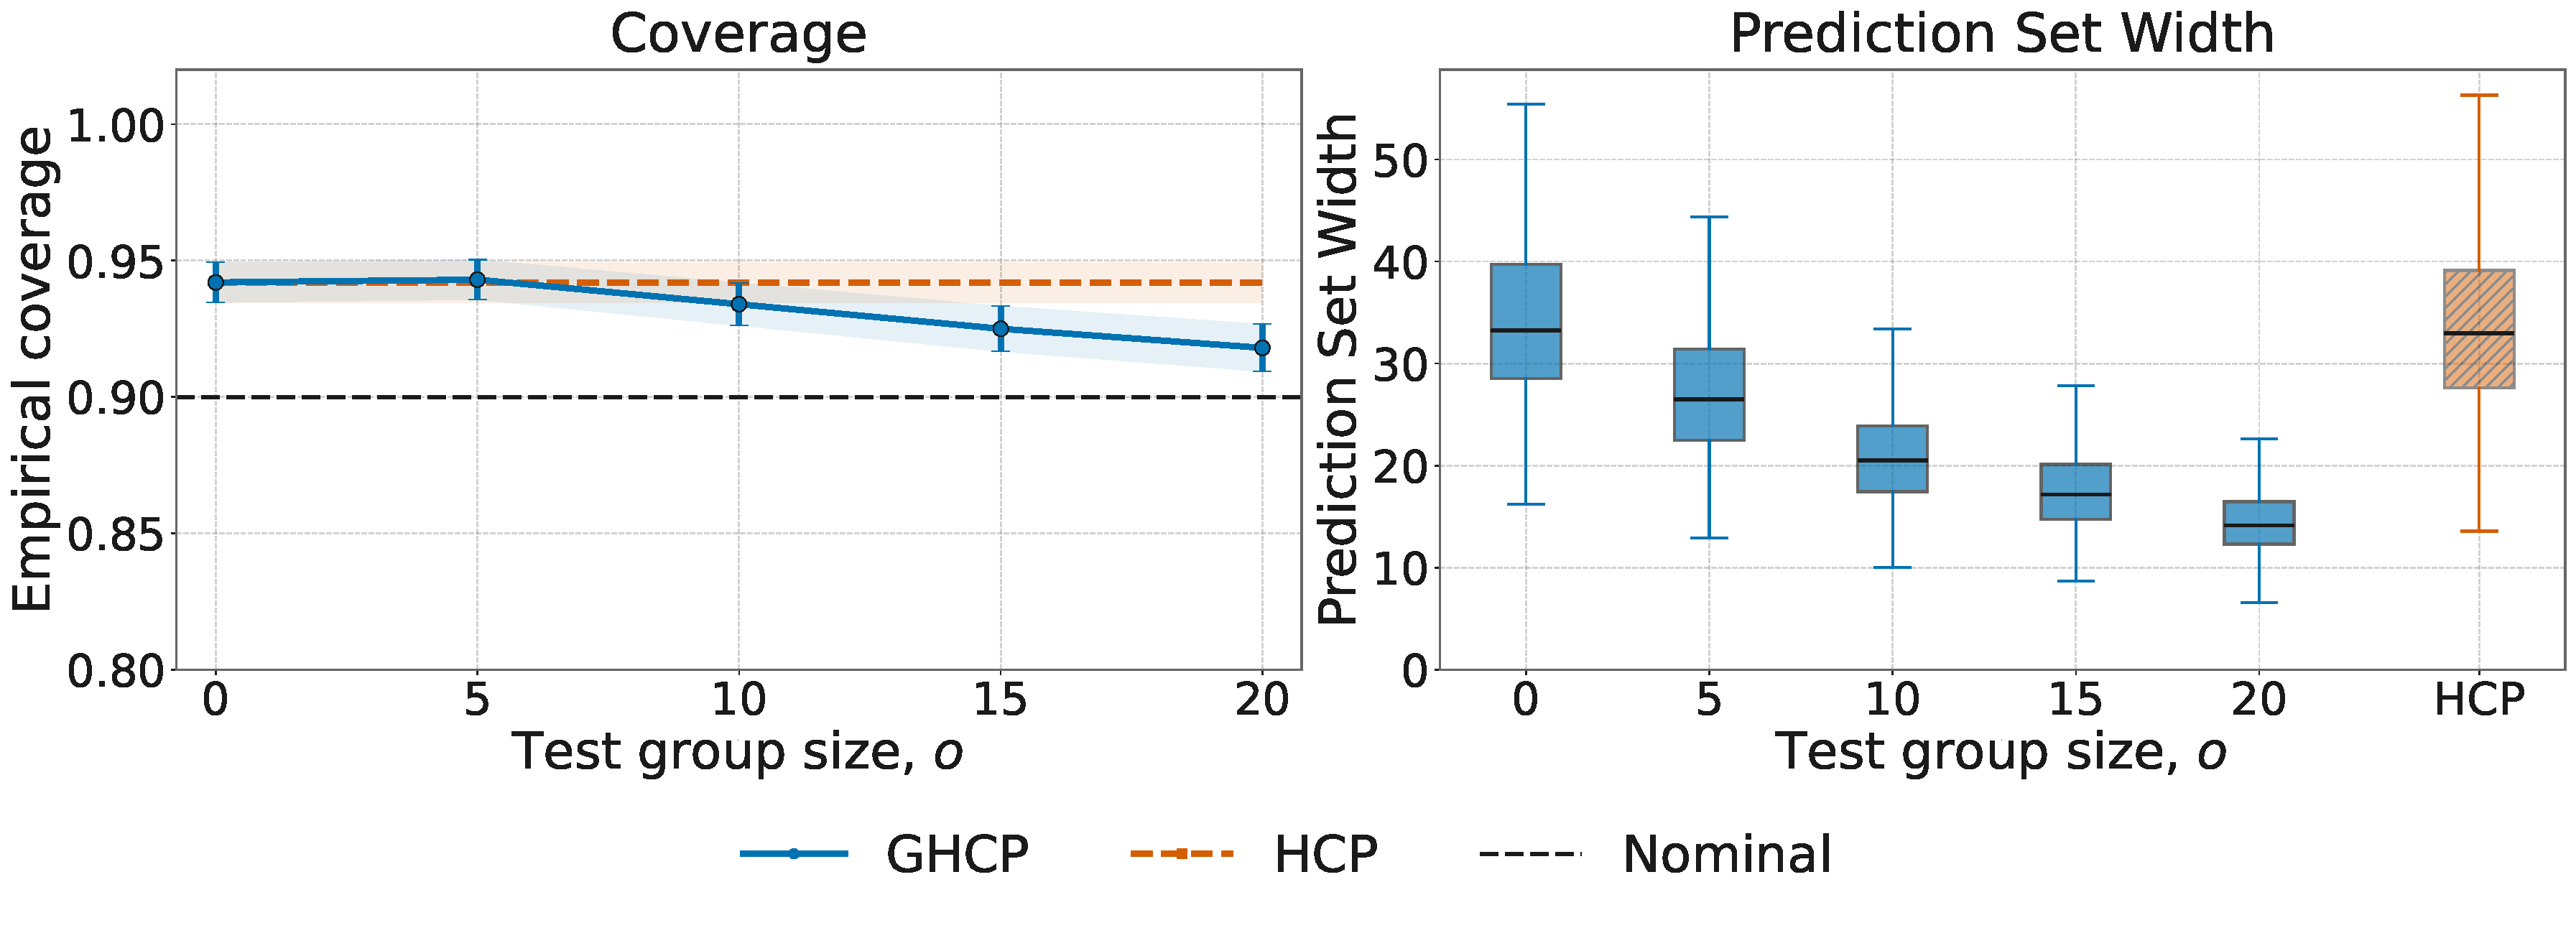
\includegraphics[width=1\linewidth]{paper-results/dgp_true_marginal_rf/figures/poisson_alpha0p1_coverage_width_by_o.pdf}
    \caption{Empirical coverage and width for HCP and GHCP with $o\in\{0,5,10,15,20\}$, using a random forest global predictor. Here $K=20$, $N_j\overset{\text{iid}}{\sim} \text{Poi}(25)$, and $\alpha=0.1$.}
    \label{fig:poi-cov-width-20}
\end{figure}

\begin{table}[t]
\centering
\caption{Empirical coverage and mean interval width for GHCP across test-group size $o$, together with HCP, for $N_j\overset{\mathrm{i.i.d.}}{\sim}\mathrm{Poi}(25)$, $\gamma=5$, and $\alpha=0.1$, using a random forest global predictor. Entries are means across $1000$ simulation repetitions, with standard errors in parentheses.}
\label{tab:dhcp-hcp-poisson-alpha01}
\small
\setlength{\tabcolsep}{6pt}
\begin{tabular}{lcccccc}
\toprule
& \multicolumn{5}{c}{GHCP} & HCP \\
\cmidrule(lr){2-6}
Value of $o$ & 0 & 5 & 10 & 15 & 20 & -- \\
\midrule
Coverage ($1-\alpha=0.90$)
& 0.967 (0.006)
& 0.946 (0.007)
& 0.941 (0.007)
& 0.914 (0.009)
& 0.925 (0.008)
& 0.944 (0.007) \\
Mean Width
& 33.824 (0.343)
& 20.897 (0.163)
& 13.407 (0.096)
& 10.323 (0.067)
& 8.699 (0.053)
& 33.775 (0.267) \\
\bottomrule
\end{tabular}
\end{table}


\subsubsection{Benefit of within-group training.}

We compare the following two versions of restricted GHCP from Algorithm \ref{alg:dhcp}, with $\eta=0.5$:
\begin{enumerate}[label=(\roman*),leftmargin=*]
    \item Restricted GHCP without within-group training. All the observations in the selected groups are used for calibration.
    \item Restricted GHCP with within-group training, using
    $\lfloor o/2\rfloor$ samples.
\end{enumerate}
\noindent  The coverage and width of the prediction sets under different values of $o$ are shown in Figure~\ref{fig:N21-wgt-vs-no-wgt} and Table \ref{tab:sim-with-vs-without-training}. We observe that within-group training helps significantly as $o$ increases. When $o=0$, GHCP with and without WGT coincide, since there are essentially no test-group samples to exploit. For $o=20$, WGT yields a $70\%$ reduction in mean width relative to no-WGT, while maintaining coverage closer to the nominal level.

\begin{figure}[h]
    \centering
    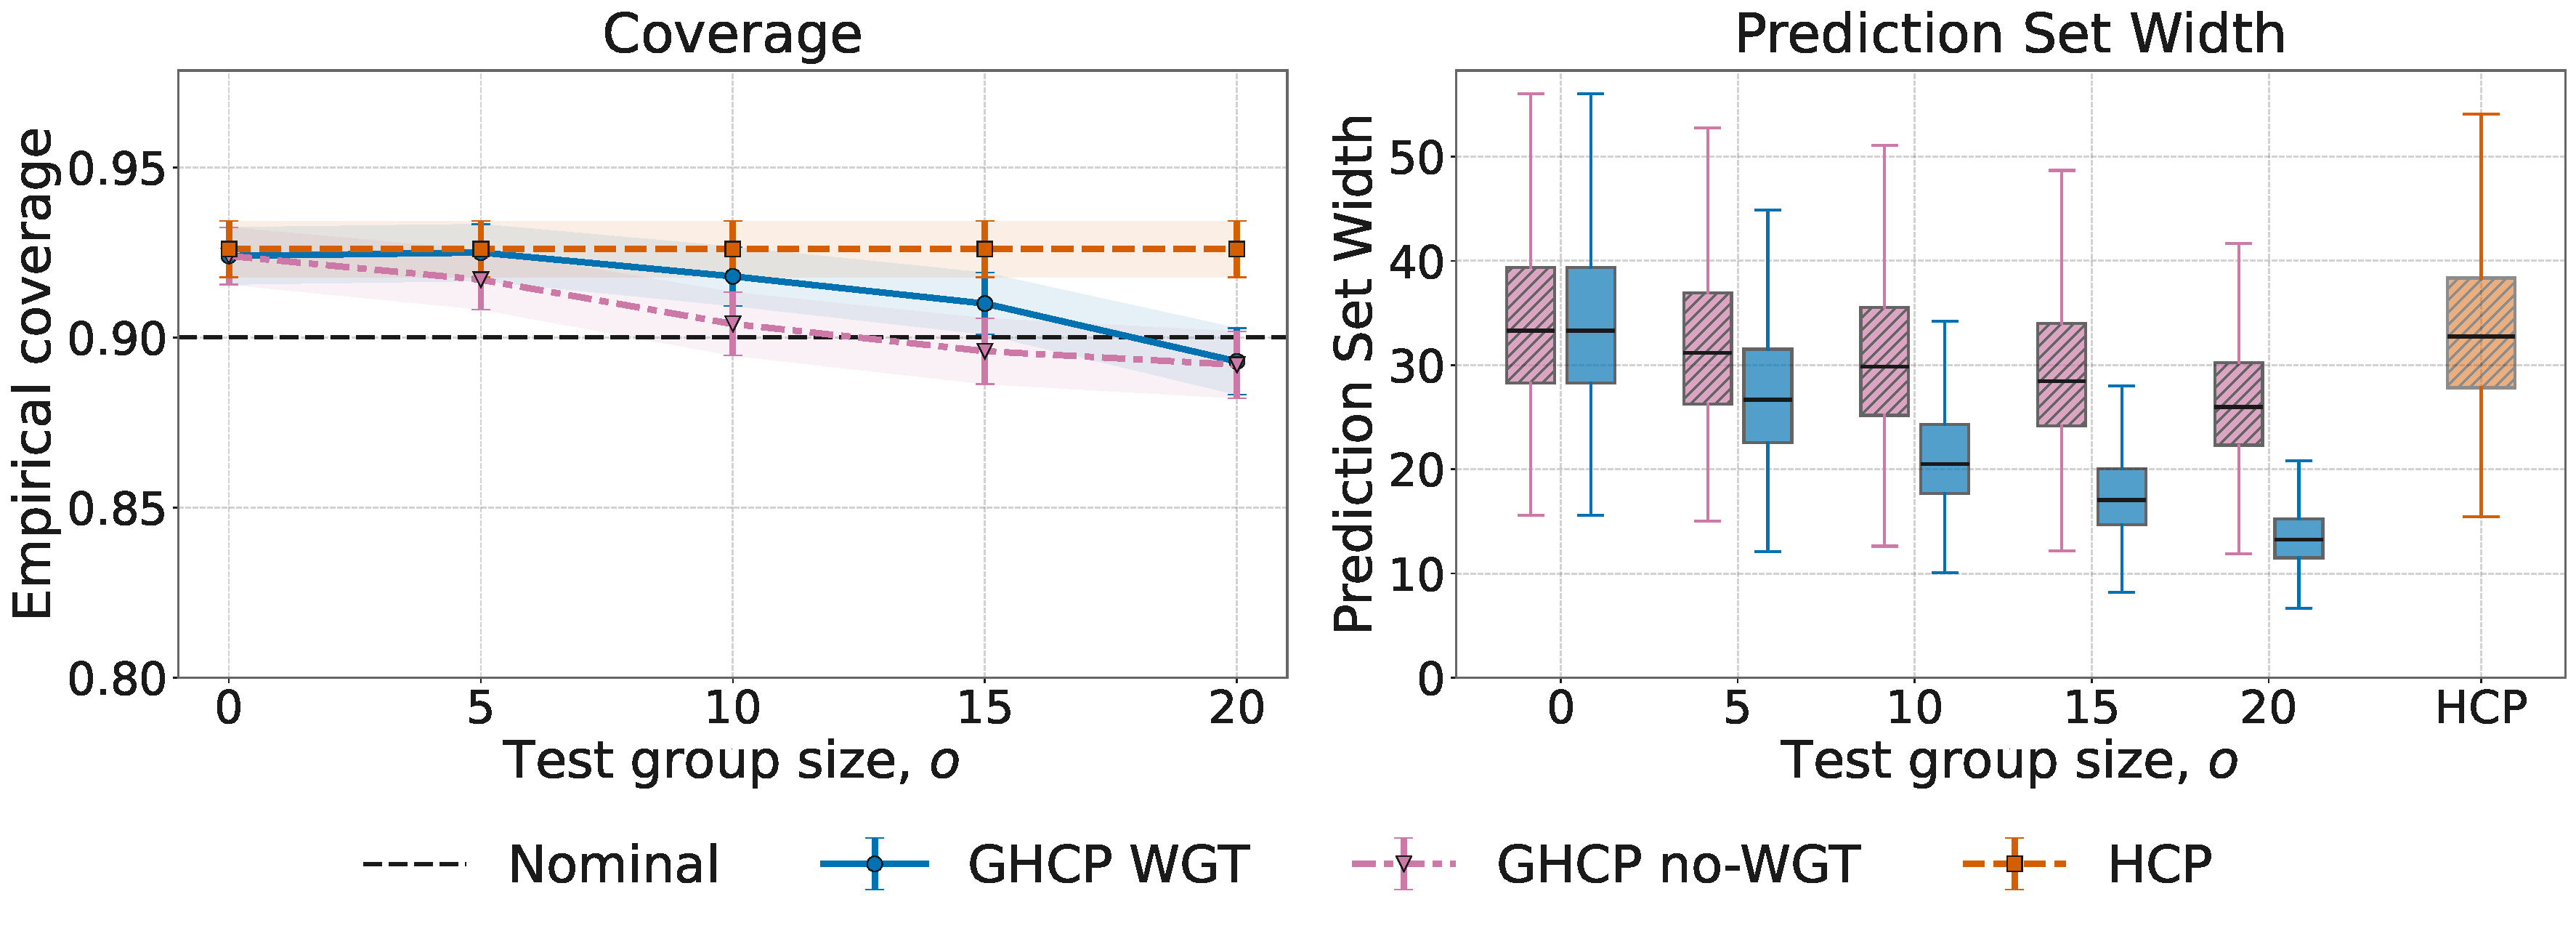
\includegraphics[width=1\linewidth]{paper-results/dgp_true_marginal_rf/figures/fixedN21_3_alpha0p1_within_vs_no_within.pdf}
    \caption{Improvement due to within-group training for $o\in\{0,5, 10, 15, 20\}$, using a random forest global predictor. Here $K=20$, $N_j\equiv 21$, and $\alpha=0.1$.}
    \label{fig:N21-wgt-vs-no-wgt}
\end{figure}

\begin{table}[t]
\centering
\caption{Empirical coverage and mean width for GHCP with and without WGT (within-group training) across test-group size $o$, together with HCP as a baseline, for fixed $N_j=21$, $\gamma=5$, and $\alpha=0.1$, using a random forest global predictor. Entries are means across $1000$ simulation repetitions, with standard errors in parentheses.}
\label{tab:sim-with-vs-without-training}
\small
\setlength{\tabcolsep}{5pt}
\begin{tabular}{llccccc}
\toprule
Metric & Method & 0 & 5 & 10 & 15 & 20 \\
\midrule
Coverage
& GHCP (no WGT) & 0.943 (0.007) & 0.936 (0.008) & 0.929 (0.008) & 0.919 (0.009) & 0.910 (0.009) \\
& GHCP (WGT)    & 0.943 (0.007) & 0.946 (0.007) & 0.942 (0.007) & 0.929 (0.008) & 0.904 (0.009) \\
& HCP            & 0.935 (0.008) & 0.935 (0.008) & 0.935 (0.008) & 0.935 (0.008) & 0.935 (0.008) \\
\addlinespace
Mean
& GHCP (no WGT) & 33.446 (0.256) & 31.433 (0.247) & 30.088 (0.241) & 28.787 (0.232) & 26.170 (0.197) \\
Width & GHCP (WGT)  & 33.446 (0.256) & 20.874 (0.151) & 13.474 (0.089) & 10.434 (0.064) & 7.925 (0.042) \\
& HCP            & 33.452 (0.260) & 33.452 (0.260) & 33.452 (0.260) & 33.452 (0.260) & 33.452 (0.260) \\
\bottomrule
\end{tabular}
\end{table}
